\chapter{Threat Model} \label{ch:threat-model}
This chapter contains the threat model established for the system under scrutiny, which was used to identify and document all threats to the system. The methodology and threat model technique is described in section \ref{ch:method:threat-modeling}.

\section{Identified Assets}
As part of the first phase of our threat modeling technique, assets of the system were identified. These can be found in table \ref{tb:assets}.
\begin{table}[!ht]
    \centering
    \begin{tabularx}{\textwidth}{r X}
        \hline
        \textbf{ID} & \textbf{Description}
        \\ \hline
        1  & Physical access to the house
        \\
        2  & Personal four-digit pin
        \\
        3  & Arm/disarm state of the system
        \\
        4  & Door contact sensor state
        \\
        5  & Authentication to the admin web application
        \\
        6  & Triggered alarm state
        \\
        7  & [TODO: Perhaps more?]
        \\ \hline
    \end{tabularx}
    \caption{The identified assets of the system}
    \label{tb:assets}
\end{table}

\section{Architecture Overview}
This section contains an architecture overview of the system. Included in this are three components presented below. First is a list of all identified use cases of the system. The second is a diagram visually presenting all components of the system, how they interact, and the data flow of the system. Lastly, a table of all identified technologies used in the system is presented.

\subsection{Use cases}
As part of the architecture overview, all use cases of the system were identified. These are the use cases a regular user would encounter when using the system normally. The use cases are documented in table \ref{tb:use-cases}.
\begin{table}[!ht]
    \centering
    \begin{tabularx}{\textwidth}{r X}
        \hline
        \textbf{ID} & \textbf{Description}
        \\ \hline
        1  & The user arms/disarms the system via the remote keypad panel
        \\
        2  & The user arms/disarms the system via the web portal
        \\
        3  & The user arms/disarms the system via the mobile app
        \\
        4  & The user receives a notification about a state change in the system
        \\
        5  & [TODO: Perhaps more?]
        \\ \hline
    \end{tabularx}
    \caption{Use cases of the system}
    \label{tb:use-cases}
\end{table}

\begin{figure}[!p]
    \centering
    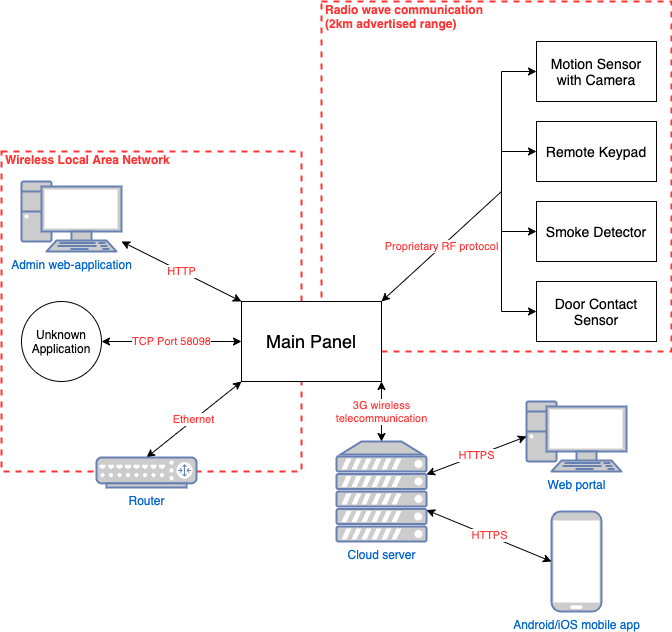
\includegraphics[width=\textwidth]{images/system-overview.png}
    \caption{Data flow diagram of the system}
    \label{fig:system-overview}
\end{figure}

\subsection{System Technologies}
Table \ref{tb:system-technologies} contains all identified technologies present in the system. There are undoubtedly additional technologies used but these are the ones identified and relevant.
\begin{table}[!p]
    \centering
    \begin{tabularx}{\textwidth}{l X}
        \hline
        \textbf{Technology}  & \textbf{Description}
        \\ \hline
        Main Panel & Linux 2.6-2.30. Hosts a web server over HTTP, using Mongoose (an embedded webserver), version unknown. Unknown application listening on TCP port 58098. Hosts DNS on TCP/UDP port 53. Has a USB and ethernet port.
        \\ \hline
        HTTP  & Protocol used by the admin web application. A clear text protocol used to communicate with the web admin panel.
        \\ \hline
        F1 RF protocol  & A proprietary \gls{RF} protocol from the hardware manufacturer, Climax Technology. Uses 868 MHz frequency. This is an undocumented protocol, meaning no technical specifications have been publicized.
        \\ \hline
        Mongoose web server  & An open-source web server, in C. Used by the main panel to host the local admin web page, version unknown. Information leaked via the HTTP \textit{Server} header on some endpoints.
        \\ \hline
        ARM architecture  & The CPU of the main panel is an ARM (little endian) SOC system from \textit{Grain Media}.
        \\ \hline
        3G telecommunication  & The main panel communicates with the external servers over the 3G mobile communication network.
        \\ \hline
        TCP  & The \gls{TCP} network protocol is used in communication. The main panel hosts three applications on different TCP ports (53, 80, 58098).
        \\ \hline
    \end{tabularx}
    \caption{Technologies used in the system}
    \label{tb:system-technologies}
\end{table}

\section{Decomposition of the system}
This section presents the results of the fourth step of the threat modeling technique. Lastly, all identified entry points of the system are listed.

\subsection{Entry points}
As part of the decomposition of the system, all entry points of the system were identified. These are essentially all points of contact an attacker could probe. The entry points are documented in table \ref{tb:entry-points}.
\begin{table}[!p]
    \centering
    \begin{tabularx}{\textwidth}{l X}
        \hline
        \textbf{Entry point} & \textbf{Description}
        \\ \hline
        Local web admin page  & See section \ref{ch:system:software}. Provides very basic functionality but no control over the system. Has an undocumented login page via \textit{HTTP Basic Auth}. Data is transferred over HTTP on the local network.
        \\ \hline
        Unknown application  & This is a completely undocumented process, listening on TCP port 58098. Closes the connection when sent data. Becomes unresponsive when sent certain data like \texttt{[]} and \texttt{\{\}} (presumably it crashes).
        \\ \hline
        Main panel  & The physical device features an Ethernet port to connect to the local network, as well as a USB port for unknown purposes. It communicates with other devices over an 868 GHz proprietary \gls{RF} protocol.
        \\ \hline
        3G telecommunication  & The device has a SIM card and communicates over the 3G telecommunication network.
        \\ \hline
        \gls{RF} communication  & The device talks to the other peripherals over a proprietary \gls{RF} protocol, called \textit{F1}\footnotelink{https://www.climax.com.tw/new/f1-features-new.php}{2021-04-02}. There seems to be little to no information available to the public about this protocol, other than its operating frequency of 868 GHz.
        \\ \hline
        USB port  & The device has a USB 2.0 Type-A connector.
        \\ \hline
        Firmware  & The firmware of the system.
        \\ \hline
    \end{tabularx}
    \caption{The entry points of the main panel}
    \label{tb:entry-points}
\end{table}

\section{Identified Threats} \label{ch:threat-model:threats}
The following section contains all identified threats. These are categorized after the threat categories of the STRIDE model. For an explanation of the model and a description of each category see section \ref{ch:method:stride}.

\subsection{Spoofing Identity}
\begin{itemize}
    \item Spoof the remote keypad.
    \item Spoof the door contact sensor.
    \item Spoof the smoke detector.
    \item Spoof the motion detection camera.
    \item Spoof the remote keypad.
    \item Spoof the admin user on the main panel.
\end{itemize}

\subsection{Tampering with Data}
\begin{itemize}
    \item Replay attack on the RF communication through message blocking via jamming.
    \item Change and tamper with RF packets in transit.
    \item Send valid RF packets to the main panel, triggering events, without proper authorization.
\end{itemize}

\subsection{Repudiation}
\begin{itemize}
    \item Replay attack on messages in the RF protocol between devices.
    \item Disrupt/disable logging of events.
\end{itemize}

\subsection{Information Disclosure}
\begin{itemize}
    \item Information leak in the packets of the \gls{RF} protocol.
    \item Insecure or non-existent encryption in the \gls{RF} protocol.
    \item Password sniffing on the local webserver.
\end{itemize}

\subsection{Denial of Service}
\begin{itemize}
    \item Jamming of the RF protocol.
    \item Stop the alarm from triggering until after you've left the premises.
    \item DoS attack on the local webserver.
    \item Crash the main panel or parts of the main panel.
    \item Crash the external devices through the RF communication.
\end{itemize}

\subsection{Elevation of Privilege}
\begin{itemize}
    \item Password attack on the local webserver login page.
    \item Send valid RF packets to the main panel without proper authorization.
    \item Gain an authenticated connection to the main panel (perhaps via the TCP 58098 application).
\end{itemize}
